\documentclass[a4paper,11pt]{article}

\usepackage[T1]{fontenc}
\usepackage{lmodern}
\usepackage{amsmath}
\usepackage{graphicx}
\setlength\abovecaptionskip{0.10ex}
\usepackage{titling}
\setlength{\droptitle}{-4cm}
\usepackage{fullpage}
\RequirePackage{graphicx}
\DeclareGraphicsExtensions{.pdf,.jpg,.png,.JPG}
\RequirePackage{float}

\usepackage{dsfont}

\newcommand{\InsertFig}[1]{
\begin{figure}[H]
\begin{center}
\includegraphics[width=.75\textwidth]{img/#1}
\end{center}
\end{figure}}
\newcommand{\InsertFigTitle}[2]{
\begin{figure}[H]
\caption{#2}
\begin{center}
\includegraphics[width=.75\textwidth]{img/#1}
\end{center}
\end{figure}}

\title{Rapport SY19 TP03 - Regle de Bayes et notion de rejet}
\author{Thomas ABASSI \& Joan MOESCH}

\begin{document}
\maketitle

\noindent Le but de ce TP est d'appr�hender la r�gle de bayes dans un probleme de detection (2 classes) dans le cas ou 3 choix sont possibles : choisir la classe 1, la classe 2 ou ne prendre aucune des 2. \\
Cette decision s'effectue grace a l'extension de la regle de Bayes (rapport des probabilites a posteriori) avec la notion de rejet. \\

\noindent Nous verrons comment s'expriment ces fonctions de decisons dans le cas general pour l'appliquer a notre probleme de detection. 

\section*{ 6. Regle de Bayes avec rejet}

\subsection*{a) Expression de la fonction de decision}
\noindent Dans le cas ou $c_{11} = c_{22} = 0$, $c_{01} = c_{02} = c_0$ et $c_{12} = c_{21} = 1$, la regle de bayes avec rejet s'ecrit : 
\begin{equation}
\delta^* (x) = \left\{ \begin{array}{ll}
a_0 & \mbox{si Min$\left( P[Y=1 | x ], P[Y = 2 | x] \right) > c_0$ }\\

a_1 & \mbox{si $ P[Y = 1 | x] > p[ Y = 2 | x]$ et $P[Y = 1 | x]  > 1 - c_0 $ } \\

a_2 & \mbox{si $ P[Y = 2 | x] > p[ Y = 1 | x]$ et $P[Y = 2 | x]  > 1 - c_0 $}\\
\end{array} \right.
\end{equation}\\

\noindent Ainsi, l'action de prendre la decision $a_1$ s'ecrit :
$$\delta^* (x) = a_1 \Leftrightarrow \left\{ \begin{array}{ll}
\mbox{$ \frac{f_1(x)}{f_2(x)} > \frac{\pi_2}{\pi_1} $ }\\
\mbox{$P[Y = 1 | x]  > 1 - c_0 $} \\
\end{array} \right.$$
 
\noindent De plus, nous avons le rapport de densite suivant :\\
   $$ 
 \begin{array}{rcl}
 \frac{f_1(x)}{f_2(x)} &=&  \displaystyle \frac{\frac{1}{2 \pi}    e^{-\frac{1}{2} (x_1 +1)^2 - \frac{1}{2} (x_2)^2}}{\frac{1}{2 \pi}    e^{-\frac{1}{2} (x_1 -1)^2 - \frac{1}{2} (x_2)^2}} \\ \\
 			       &=& \displaystyle \frac{e^{-\frac{1}{2} (x_1 +1)^2}}{e^{-\frac{1}{2} (x_1 -1)^2}} \\ \\
			       &=& \displaystyle \frac{e^{-\frac{1}{2}(x_1^2 + 2x_1 + 1)}}{e^{-\frac{1}{2}(x_1^2 -2x_1 +1)}} \\ \\
			       &=& e^{-2x_1}\\
	      \end{array}
   $$

\noindent En rappelant que la probabilite a posteriori est donnee par  :
\begin{equation}
P[Y = 1 | x ] = \frac{\pi_1 f_1(x)}{\pi_1 f_1(x) + \pi_2 f_2(x)}
\end{equation}\\

\noindent Nous obtenons donc :
$$\delta^* (x) = a_1 \Leftrightarrow \left\{ \begin{array}{ll}
\mbox{$ e^{-2x_1} > \frac{\pi_2}{\pi_1} $}\\
\mbox{$\frac{\pi_1 f_1(x)}{\pi_1 f_1(x) + \pi_2 f_2(x)} > 1 - c_0 $} \\
\end{array} \right.$$\\

\noindent Ce qui nous donne finalement l'expression de la regle en fonction de $x_1$ : 

\begin{equation}
\delta^* (x) = a_1 \Leftrightarrow \left\{ \begin{array}{ll}
\mbox{$ x_1 < - \frac{1}{2}Ln(\frac{\pi_2}{\pi_1})$}\\
\mbox{$ x_1 < -\frac{1}{2} Ln(\frac{\pi_2}{\pi_1} \frac{1 - c_0}{c_0}) $} \\
\end{array} \right.
\end{equation}

\noindent De la meme maniere, nous trouvons les equations de frontiere pour la classe $\omega_2$ : 

\begin{equation}
\delta^* (x) = a_2 \Leftrightarrow \left\{ \begin{array}{ll}
\mbox{$ x_1 > - \frac{1}{2}Ln(\frac{\pi_2}{\pi_1})$}\\
\mbox{$ x_1 > -\frac{1}{2} Ln(\frac{\pi_2}{\pi_1} \frac{c_0}{1 - c_0}) $} \\
\end{array} \right.
\end{equation}

\noindent La droite d'equation $x = - \frac{1}{2}Ln(\frac{\pi_2}{\pi_1})$ correspond au centre de la zone de rejet, commune aux deux equations de frontieres pour $a_1$ et $a_2$.\\
D'autre part, les droites d'equations  $ x_1 = -\frac{1}{2} Ln(\frac{\pi_2}{\pi_1} \frac{1 - c_0}{c_0})$ et $x_2 = -\frac{1}{2} Ln(\frac{\pi_2}{\pi_1} \frac{c_0}{1 - c_0})$  correspondent respectivement aux frontieres extremes de la zone de rejet, dans le cas ou l'on choisit la classe $\omega_1$ ou $\omega_2$.\\
\\

\subsection*{b) Traces des frontieres}
\noindent Nous ecrivons la fonction suivante : \\

\noindent $bayesRejet <- function( n, pi1, pi2, L0)$

	$x0 = - log( pi2 / pi1 ) / 2$
	
	$x1 = - 1/2 * log( pi2 * (1 - L0) / (pi1 * L0) )$
	
	$x2 = - 1/2 * log( pi2 * L0 / (pi2 * (1-L0) ) )$

	$echantillon(n)$
	
	$abline(v= x0, col= "red")$
	
	$abline(v= x1, col ="blue")$
	
	$abline(v= x2, col ="green")$ \\

\noindent Ou la fonction $echantillon$ trace le nuage de points en coloriant chaque individus selon sa classe. Pour chaque cas, voici les resultats obtenus :

\subsubsection*{Cas 1} Nous prenons les valeurs $\pi_1 = \pi_2$, $c_0 = 0.4$
\begin{center}  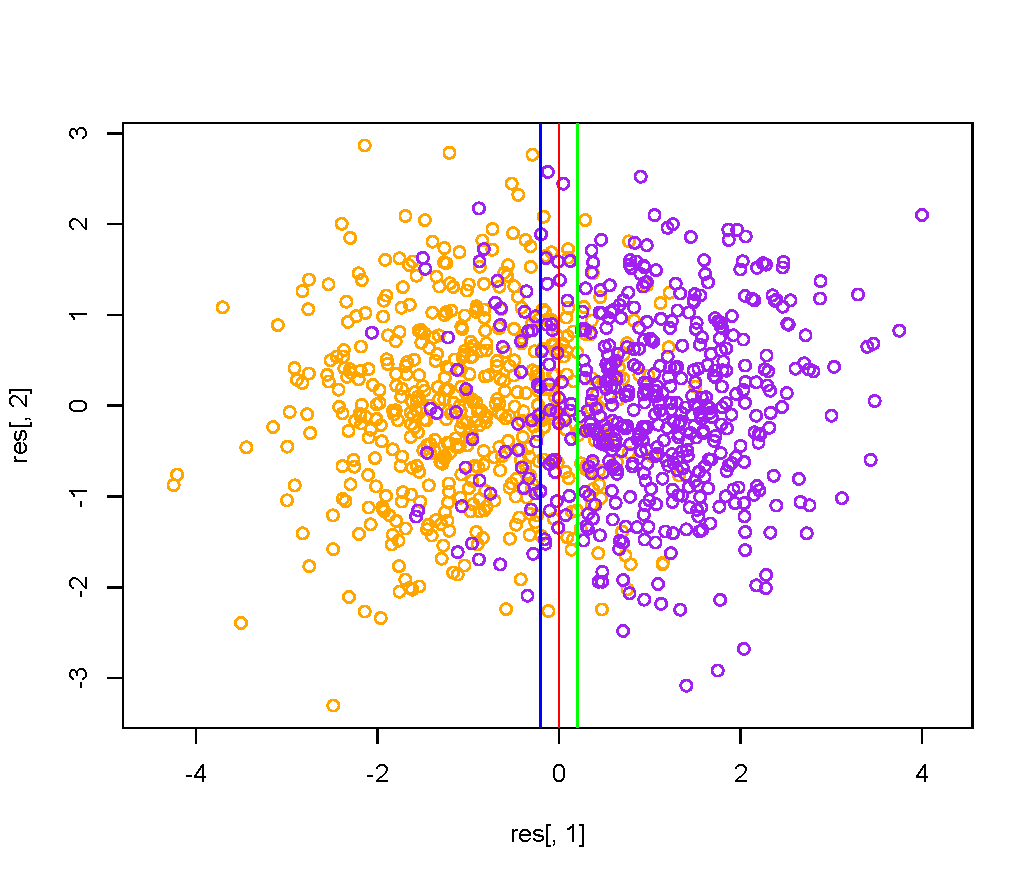
\includegraphics[width=0.6\textwidth]{rejet_1.pdf} \end{center}
\subsubsection*{Cas 2} Nous prenons les valeurs $\pi_1 = \pi_2$, $c_0 = 0.1$
\begin{center}  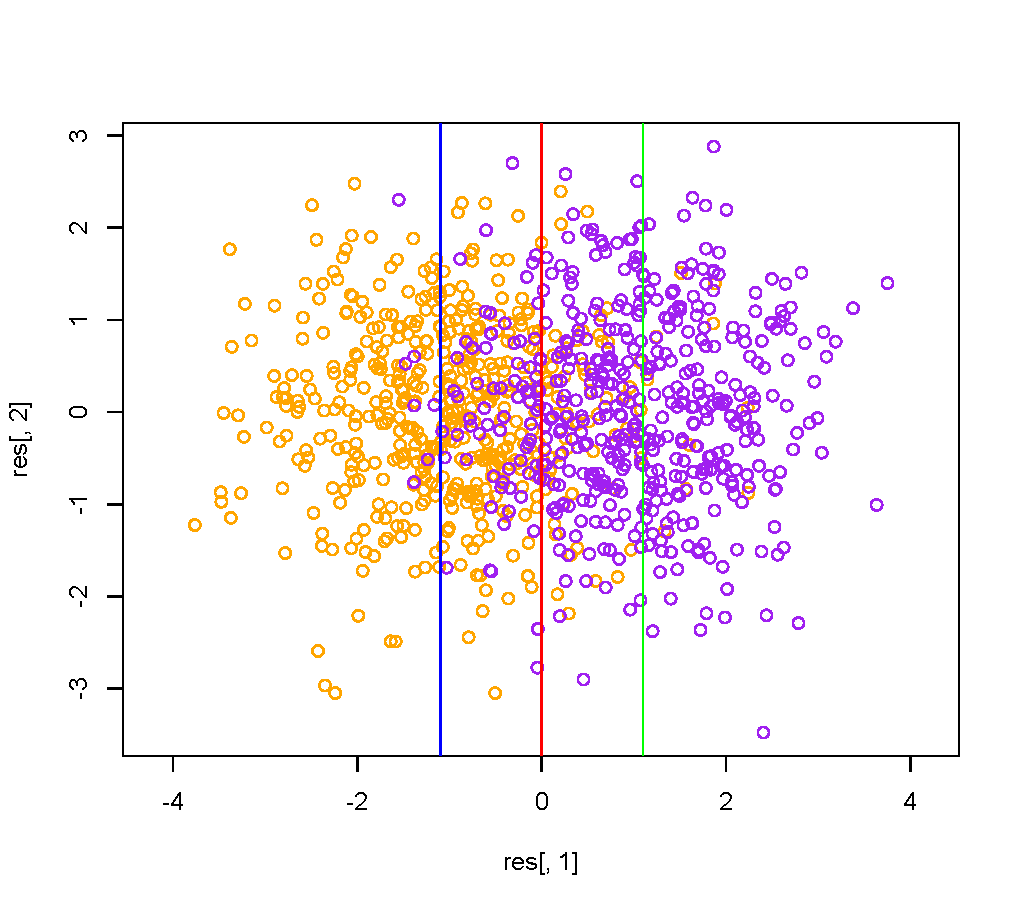
\includegraphics[width=0.6\textwidth]{rejet_2.pdf} \end{center}
\noindent Dans chaque cas, les donnnes � gauche de la droite bleu sont classees dans $w_1$, ceux � droite de la verte dans $w_2$ et aucune classe n'est attribuee dans le cas des donnees entre la bleu et la rouge. La droite rouge represente l'axe central de la zone de rejet.\\

\noindent On remarque que plus le cout de rejet $c_0$ est faible, plus la zone de rejet a tendance � s'agrandir. Ceci entrainera evidemment une baisse de l'erreur de decision mais provoquera egalement une baisse du nombre de decisions (plus de rejet).\\

\subsection*{c) Estimation des erreurs de decision}
\noindent Par definition, les probabilites de mauvaises decisions $\alpha$ et $\beta$ sont donnes par :

$ \alpha = P( \delta^*(X) = a_2 | \omega_1 ) $

$ \beta = P( \delta^*(X) = a_1 | \omega_1 ) $\\

\noindent On peut donc estimer ces deux types d'erreurs en comptant le nombre d'individus de la classe $\omega_1$ qui ne sont a droite de "l'axe vert" et le nombre d'individus de la  classe $\omega_2$ qui ne sont � gauche de "l'axe bleu".\\

\noindent En posant $x_1$ et $x_2$ les abcisses des droites bleue et verte (extremites de la zone de rejet), les estimateurs s'ecrivent:

$ \hat\alpha =  \frac{1}{n_1}\sum_{\omega_1}\mathds{1}_{x_i > x_2}(i)$

$ \hat\beta =  \frac{1}{n_2}\sum_{\omega_2}\mathds{1}_{x_i < x_1}(i)$\\

\noindent Dans le cas $c_0 = 0.4$, nous obtenons les valeurs d'erreurs de classification suivantes :

$ \hat\alpha =  0.126$

$ \hat\beta =  0.106$\\

\noindent Dans le cas $c_0 = 0.1$, nous obtenons les valeurs d'erreurs de classification suivantes :

$ \hat\alpha =  0.02$

$ \hat\beta =  0.014$\\

\noindent La valeur du seuil de rejet permet donc de diminuer les erreurs de classification.\\
\\

\subsection*{d) Probabilites de rejet et d'erreur}
\noindent La probabilite de rejet de la decision correspond a la quantite des individus qui se trouvent dans la region de rejet, c'est a dire entre $x_1$ et $x_2$, un bon estimateur de cette probabilite serait donc :\\

$ \hat r =  \frac{1}{n}\sum_{i=1}^n \mathds{1}_{x_1 < x_i < x_2}(i)$\\

\noindent Ceci nous donne, dans le cas $c_0 = 0.4$, une estimation :

$ \hat r = 0.098$\\

\noindent Dans le cas $c_0 = 0.1$, nous avons :

$ \hat r = 0.538$\\

\noindent Ceci confirme bien les theories avancees precedemment : plus le cout $c_0$ est faible, plus les erreurs $\alpha$ et $\beta$ diminuent mais plus la probabilite de rejet augmente. Ceci est facilement comprehensible dans le sens ou la region de rejet augmente lorsque la valeur de $c_0$ diminue.\\
\\

\noindent D'autre part, l'estimateur de la probabilite d'erreur est donne par :  $\epsilon( \delta^* ) = \frac{\hat\alpha + \hat\beta}{n_1 + n_2}$\\

\noindent Nous obtenons donc l'estimation de la probabilite d'erreur : 

Dans le cas $c_0 = 0.4$, $\hat\epsilon(\delta^*) = 2.32 . 10^{-4}$

Dans le cas $c_0 = 0.1$, $\hat\epsilon(\delta*) = 0.34 . 10 ^{-4}$

\end{document}